\documentclass[a4paper,12pt]{article}
\usepackage[english,ukrainian,russian]{babel}
\linespread{1}
\usepackage{ucs}
\usepackage[utf8]{inputenc}
\usepackage[T2A]{fontenc}
\usepackage[paper=portrait,pagesize]{typearea}
\usepackage{amsmath}
\usepackage{bigints}
\usepackage{amsfonts}
\usepackage{graphicx}
\usepackage{amssymb}
\usepackage{cancel}
\usepackage{gensymb}
\usepackage{ragged2e}
\usepackage{multirow}
\usepackage{rotate} 
\usepackage{pdflscape}
\usepackage{bigstrut}
\usepackage[pageanchor]{hyperref}
\usepackage{svg}
\usepackage{chngpage}
\newcommand{\dx}{\textbf{d}x}
\newcommand{\dt}{\textbf{d}t}
\newcommand{\du}{\textbf{d}u}
\newcommand{\dv}{\textbf{d}v}
\newcommand{\dy}{\textbf{d}y}
\newcommand{\ds}{\textbf{d}s}
\newcommand{\dz}{\textbf{d}z}
\newcommand{\arch}{\textrm{arcch}}
\newcommand{\arsh}{\textrm{arcsh}}
\newcommand{\dint}{\displaystyle\int}
\newcommand\tab[1][1cm]{\hspace*{#1}}
\newcommand{\dsum}{\displaystyle\sum}
\usepackage[left=20mm, top=20mm, right=15mm, bottom=15mm, nohead, nofoot]{geometry}
\newcommand{\ri}{R_i}
\newcommand{\re}{R_e}
\newcommand{\uo}{U_0}
\newcommand{\ik}{I_{kz}}
\newcommand{\po}{P_0}
\newcommand{\pio}{P_i}
\newcommand{\pe}{P_e}




\begin{document}

\begin{justify}
		\thispagestyle{empty}\setlength{\parindent}{0pt}
	\begin{center}
		\textbf{НАЦІОНАЛЬНИЙ ТЕХНІЧНИЙ УНІВЕРСИТЕТ УКРАЇНИ}\\ 
		\textbf{«КИЇВСЬКИЙ ПОЛІТЕХНІЧНИЙ ІНСТИТУТ»}\\ 
		\textbf{ФІЗИКО-ТЕХНІЧНИЙ ІНСТИТУТ}
	\end{center}
	$\\\\\\\\\\\\\\\\\\\\\\\\\\$
	\begin{center}
		Лабораторна робота з фізики №3\bigbreak
КОНДЕНСАТОР І ІНДУКТИВНІСТЬ В КОЛІ ЗМІННОГО СТРУМУ
	\end{center}
	$\\\\\\\\\\\\\\\\\\\\\\\\\\$
	\begin{flushright}
	Виконалa:\\
		студент групи ФІ-12\\
		Бекешева Анастасія 
	\end{flushright}
	$\\\\\\\\\\$
	\begin{center}
		\textbf{Київ-2022}
	\end{center}
	\newpage





\newpage
	\begin{center}
		\section* {РОЗДІЛ ПЕРШИЙ\\ТЕОРЕТИЧНА ДОВІДКА }
	\end{center}
    \subsection*{Частина 1: Ємність в колі змінного струму.}
	\textit{\textbf{Ключові поняття:} Змінний струм, ємність, конденсатор, правила Кірхгофа для змінного струму, 
    стала часу, паралельне з’єднання, послідовне з'єднання, імпеданс, фазовий зсув, векторна діаграма, теорема Фур’є.}
	\begin{center}
		\textbf{Мета роботи}
	\end{center}

    Визначення реактивного опору конденсатора як функції частоти та його ємності. 
    Визначення фазового зсуву між напругою на конденсаторі та струмом у колі як функції частоти та ємності конденсатора.
    \begin{center}
		\textbf{Теоретичне підгрунтя }
	\end{center}

    Розглянемо конденсатор та дві пластини (А) та (В), що розділені діелектриком (рис. 1).
    \begin{figure}[h!]
		\begin{center}
			%\includegraphics[scale=0.8]{Shema_1.jpg}
		\end{center}
		\caption{Схема під’єднання конденсатора.}
		\label{Picture_1}
	\end{figure}

    Оскільки пластина (В) знаходиться під потенціалом землі, різниця потенціалів, що приходиться на конденсатор, дорівнює потенціалу $\varphi_A$ пластини (А) і
    пов'язана з кількістю електрики $Q_A$ на пластині (А) так:
    $$Q_A=C\cdot\varphi_A \eqno(1)$$
    де $C$ - – ємність конденсатора.

    Якщо замкнути ключ $Р$ (рис. 1), через резистор $R$ потече струм:
    $$R=\dfrac{\varphi_R}{R} \eqno(2)$$
    З правила Кіргофа витікає, що $\varphi_K=-\varphi_C$. Тому $I=-\dfrac{\varphi_C}{R}$
    З іншого боку диференціюючи (1), отримаємо
    $$I=\dfrac{C\cdot d\varphi}{\dt} \eqno(3)$$
    Тобто, струм розряду пропорційний зменшенню заряду конденсатора і, відповідно, його потенціалу. 
    Порівнюючи (1) та (3) отримаємо:
    $$\dfrac{d\varphi}{\dt}=-\dfrac{1}{RC\cdot\varphi} \eqno(4)$$
\newpage
    Шляхом розділення змінних диференційне рівняння (4) розв'язується як:
    $$\varphi=\varphi_0\cdot e^{-t/RC} \eqno(5)$$
    де $\varphi_0$ – початковий потенціал конденсатора.

    Величина $\tau =RC$ має розмірність часу і називається сталою часу RС –кола. 
    Вона відповідає характерному часу розрядки конденсатора С через резистор $R$
    \begin{figure}[h!]
		\begin{center}
			%\includegraphics[scale=0.8]{Shema_2.jpg}
		\end{center}
		\caption{Схема зарядки конденсатора.}
		\label{Picture_2}
	\end{figure}

    Розглянемо процес зарядки конденсатора (рис. 2). Повторюючи викладки, 
    які наведені вище, і враховуючи джерело ЕРС в рівнянні Кіргофа $U_R+U_C+E_0=0$, отримаємо
    $$\varphi=E_0(1-e^{-t/RC}) \eqno(6)$$

    Отже процес зарядки конденсатора протікає з тією ж швидкістю, що і розрядки.

    Знайдемо тепер енергію конденсатора. Істотно, що в міру зарядки конденсатора його потенціал змінюється. Додавання конденсатору з 
    потенціалом невеликої кількості електрики змінює його енергію на $dW=\varphi dQ$.
    Інтегруючи від 0 до $Q_0$, отримуємо повну енергію:
    $$W=\dfrac{1}{2}\cdot\dfrac{Q_0^2}{C}=\dfrac{1}{2}CE_0^2 \eqno(7)$$

    З іншого боку повна робота, що виконується джерелом напруги дорівнює $E_0Q_0=CE_0^2$.

    Вищенаведені міркування вказують на те, що можна говорити про струм через 
    конденсатор так само, як і через резистор або через індуктивність. Єдина відмінність 
    полягає в іншому вигляді зв'язку між струмом через конденсатор та потенціалом на 
    його обкладинках. До того ж цей звя’зок варто розглядати тільки в колах зі змінною напругою.

    Розглядемо схеми, в яких джерело напруги генерує гармонічний сигнал, 
    тобто ЕРС елементу змінюється з часом періодично з частотою . Різниця 
    потенціалів на обкладинках конденсатора при певному струмі буде тим менше, чим 
    більше частота. При збільшенні частоти зменшується час протягом якого струм, 
    зберігаючи свій напрямок, буде заряджати або розряджати конденсатор. Тому, як 
    видно з (5), зі збільшенням частоти зменшується заряд, до якого встигає 
    зарядитись конденсатор, а, отже, і потенціал на його обкладинках. Друга 
    особливість полягає в тому, що максимальному струмові відповідає максимальна 
    зміна напруги на обкладинках конденсатора. Викладемо ці ж міркування в 
    математичній формі.

    Зручно представити потенціал на обкладинках конденсатора в комплексному вигляді:
    $$\varphi=\varphi_0exp(i\omega t+\psi_0)=\varphi_0\lfloor \cos(\omega t+\psi_0)+i\sin(\omega t+\psi_0)\rfloor \eqno(8)$$
    де $\varphi_0$ та $\psi_0$ амплітуда та початкова фаза потенціалу.
\newpage
    Підставляючи (8) в (3) для струму отримаємо:
    $$I=i\omega C\cdot\varphi_0exp(i\omega t+\psi_0)=i\omega C\cdot\varphi \eqno(9)$$
    Величину
    $$Z_c=\dfrac{1}{i\omega C} \eqno(10)$$
    називають імпедансом конденсатора. Підставляючи в (9) отримаємо 
    зв’язок між струмом через конденсатор та потенціалом на його обкладинках у вигляді закону Ома:
    $$I=\varphi\cdot Z_c \eqno(11)$$

    Як перше та і друге правило Кірхгофа можна застосовувати до змінних струмів, 
    якщо омічний опір всюди замінити на відповідний імпеданс.

    Зв’язок між струмом та потенціалом конденсатора зручно представити в вигляді 
    \textbf{векторної діаграми}. В будь який момент струм (9) можна представити в вигляді 
    вектора, що обертається з частотою . При цьому вектор струму (8) випереджає 
    вектор потенціалу на пів періоду. Зсув фаз між вектором струму та вектором 
    потенціалу (напруги) через конденсатор становить $\dfrac{\pi}{2}$.

    Розглянемо тепер зв’язок між напругою та струмом в колі з послідовно з’єднаними 
    конденсатором та резистором (рис. 2). Скориставшись правилами Кірхгофа для кола зі змінним струмом отримаємо: 
    $$U_i=I\cdot R+\dfrac{I}{i\omega C}=I\bigg(R+\dfrac{1}{i\omega C}\bigg) \eqno(12)$$

    Якщо вхідний сигнал можна представити в вигляді $U_{in}=U_0\cos(\omega t)$, користуючись (12) неважко знайти струм в колі:
    $$I=\dfrac{U_{in}}{\bigg(R+\dfrac{1}{i\omega C}\bigg)}=I_0\cos(\omega t+\phi) \eqno(13)$$

    де – $\phi$ зсув фаз між вхідною напругою та струмом в RC-колі:
    $$\tg(\phi)=-\dfrac{1}{\omega R C} \eqno(14)$$
    $I_0$ - амплітуда струму:
    $$I_0=\dfrac{U_0}{\sqrt{R^2+\dfrac{1}{\omega^2 C^2}}} \eqno(15)$$
    Загальний імпеданс RC кола становить:
    $$Z=\dfrac{U_0}{I_0}=\sqrt{R^2+\dfrac{1}{\omega^2 C^2}} \eqno(16)$$

    Якщо прийняти до уваги, що напруга на резисторі пропорційна струму, то на 
    векторній диаграмі струм в колі можна представити у вигляді вектора зсунутого на 
    кут $\phi$ відносно вектора вхідної напруги.
\newpage
    Яким же чином буде змінюватись струм в RC-колі за довільної форми вхідного 
    сигналу? Це питання визначає теорема Фурьє, згідно з якою будь-який сигнал можна 
    представити у вигляді ряду гармонічних сигналів:
    $$U_{in}(t)=\sum\limits_{\omega_{min}}^{\omega_{max}}A_0\cdot exp\{\omega t\} \eqno(17)$$

    Тоді, з огляду на принцип суперпозиції, до кожної з гармонічних складових сигналу 
    (17) можна застосувати формули (12 – 16). Отже:
    $$I(t)=\sum\limits_{\omega_{min}}^{\omega_{max}}\dfrac{A_\omega}{R+\dfrac{1}{i\omega C}}\cdot exp\{\omega t\} \eqno(18)$$

    З (18) випливає, що в загальному випадку вхідний сигнал може в значній мірі 
    спотворюватися RC-колом. Однак, в деяких випадках такі схеми працюють доволі 
    прозоро. Розглянемо рис. 3. Вихідний сигнал:
    $$U_{out}=\dfrac{\dint I\cdot\dt}{C}=\dfrac{\dint U_{in}\cdot\dt}{C\bigg(R+\dfrac{1}{i\omega C}\bigg)} $$

    За умов коли $R>>\bigg|\dfrac{1}{\omega C}\bigg|$ на рис. 3 працює як інтегратор, тобто вихідний сигнал є інтеграл від вхідного:
    $$U_{out}=\dfrac{\dint I\cdot\dt}{C}=\dfrac{\dint U_{in}\cdot\dt}{RC}=\dfrac{\dint U_{in}\cdot\dt}{\tau} \eqno(19)$$

    Умова інтегрування фактично означає, що характерний час заряду конденсатора має 
    бути набагато більше періоду найвисокочастотнішої компоненти вхідного сигналу. Для кола на рис. 3 вихідний сигнал:
    $$U_{out}=I\cdot R=R\cdot\dfrac{dQ}{\dt}=RC\cdot\dfrac{dU_c}{\dt}=\tau\cdot\dfrac{d(U_{in}-U_R)}{\dt}$$

    За умов коли $|U_{in}|>>|U_R|$ вихідний сигнал є диференціалом вхідного, тобто коло працює як таке, що диференціює:
    $$U_{out}=\tau\cdot\dfrac{dU_{in}}{\dt} \eqno(20)$$

    З умови $|U_{in}|>>|U_R|$ безпосередньо слідує, що $|U_C|>>|U_R|$, отже, і імпеданс 
    конденсатора набагато більший за опір $\bigg|\dfrac{1}{\omega C}\bigg|>>R$. Іншими словами 
    час розрядки конденсатора набагато менше періоду низькочастотної компоненти вхідного сигналу.

\newpage
	\begin{center}
		\section* {РОЗДІЛ ДРУГИЙ\\Теоретичні основи експерименту}
	\end{center}
    Схему установки для дослідження RC-кола наведено на рис. 3.
    \begin{figure}[h!]
		\begin{center}
			%\includegraphics[scale=0.6]{Shema_3.jpg}
		\end{center}
		\caption{Схема дослідження RC–кола.}
		\label{Picture_3}
	\end{figure}

    Вона складається з монтажної коробки, диференціальних повторювачів, 
    осцилографа та генератору ГЗ-11/1. RC-коло монтується на монтажній коробці з 
    набору резисторів (50; 100; 200 Ом) та конденсаторів. Низькочастотний генератор 
    синусоідального сигналу використовується для визначення імпедансу кола. Та 
    дозволяє вивчити особливості роботи диференціюючого та інтегруючого кола. 

    Диференціальний підсилювач викристовуються для одночасного вимірювання 
    двох напруг при підключенні до входів двоканального осцилографа. Його входи 
    можуть бути підключені до будь-якої точки кола не впливаючи на його електричну поведінку.

    Він має два входи, які позначені літерами (A) та (B), кожен з яких має пару 4 мм 
    сокетів червоного та синього кольору. В роботі використовується двохканальний 
    осцилограф, що дозволяє одночасно вивчати сигнал на резисторі та конденсаторі. 
    Осцилограф може працювати в двох режимах. В режимі осцилографа можна 
    спостерігати часову розгортку досліджуваних сигналів. Зсув фаз вимірюється 
    безпосередньо на осцилографі за допомогою маркера на синхронізованих 
    синусоїдах сигналу генератора та напруги на резисторі. Тангенс зсуву фаз 
    обчислюється відносно амплітуд напруги на резисторі та конденсаторі.

    В режимі осцилоскопа на канал "А" подається сигнал від резистора 
    (пропорційний струму в колі); на канал "В" - сигнал від конденсатора чи 
    безпосередньо від генератора. На екрані при цьому спостерігаються фігури Ліссажу. 
    Форма фігури залежить від зсуву фаз між сигналами, що подаються на вхід "А" та 
    "В". Так, якщо на вхід "В" подається сигнал від конденсатора, то спостерігається еліпс:
    \begin{center}
        канал "А" (вісь X): $X=I_0\cos(\omega t+\phi_0)$ \\
        канал "В" (вісь У): $Y=I_0\sin(\omega t+\phi_0)$
    \end{center}
    Звідки, виключивши $t,\: y=\biggl(\dfrac{1}{C\omega}\biggr)\cdot I_0\cdot\sin(\omega t+\phi_0)$ отримуємо формулу еліпсу:
    $$\biggl(\dfrac{x}{I_0}\biggr)^2+\biggl(\dfrac{y}{\frac{I_0}{C\omega}}\biggr)=1$$
    Якщо на канал "В" подається вхідний сигнал, осі еліпса вже не співпадають з осями $X$ та $Y$.

\newpage
    \begin{center}
		\textbf{Хід експерименту}
	\end{center}
    \begin{enumerate}
        \item Зберіть схему, як показано на рис. 3.
        \item Візьміть конденсатор ємністю 1$\mu$Ф, резистор з найменшим опором. За допомогою 
        ручки генератора підберіть частоту, коли амплітуда напруги на конденсаторі (канал "B") 
        дорівнюватиме амплітуді напруги на резисторі (канал "A"). Це також означає, що при цій частоті $X_C=R$.
        \item Поступово збільшуйте опір резисторів (10, 15, 25, 50, 75, 100, 150, 200 Ом) і 
        знімайте залежність $X_C=f(\nu)$. Перемикніть осцилограф в режим осцилоскопа, переконайтесь, що ви бачите коло на екрані.
        \item Візьміть конденсатор ємністю $2,2\mu$Ф. Повторіть вимірювання як зазначено в п. 3, 
        після чого візьміть конденсатор ємністю $4,4\mu$Ф і також повторіть п.3.
        \item Візьміть конденсатор ємністю 1 мкФ та резистор опором 50 Ом. Змінюючи 
        частоту генератора в межах п. 3 вимірюйте відношення амплітуди напруги на 
        конденсаторі $U_{0C}$ до амплітуди напруги на резисторі $U_{0R}$. Відношення цих амплітуд 
        є тангенсом зсуву фаз між струмом в колі та напругою генератора.
        $$\tg\varphi=\dfrac{U_{0C}}{U_{0R}}$$
    \end{enumerate}

    Даний пункт можна виконати також/або теоретично, взявши весь ряд значеннь 
    реактивних опорів, та підставивши значення активного опору 50 Ом, розрахувати:
    $$\tg\varphi=-\dfrac{X_C}{R}$$
    \begin{center}
		\textbf{Завдання}
	\end{center}
    \begin{enumerate}
        \item За результатами вимірювання побудуйте отримані залежності $X_C=f(\nu)$ в лінійних 
        та логарифмічних координатах для всіх випадків. Зробіть це на одній координатній площині. Апроксимуйте дані теоретичною залежністю.
        \item Зробіть зріз апроксимованих залежностей, побудованих в п. 1 для кількох частот 
        і побудуйте залежність імпедансу від ємності $X_C=f(C)$. З параметрів апроксимації 
        визначте показник виконання залежності.
        \item Побудуйте залежність зсуву фаз від частоти згідно п.5.
        \item Зробіть висновки.
    \end{enumerate}
    \newpage
    \begin{center}
    	\section* {РОЗДІЛ ТРЕТІЙ\\}
    \end{center}
    \subsection*{Частина 1}
    \begin{figure}[h!]
		\begin{center}
			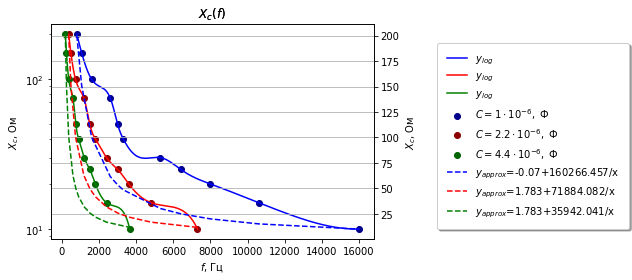
\includegraphics[scale=0.8]{media/graph13a}
		\end{center}
		\caption{Графік залежності опору від частоти}
		\label{Picture_1}
	\end{figure}
	За допомогою формули (1) розрахуємо $C$ апроксимоване:
	\begin{equation}
		C_{\textrm{апр}}=\dfrac{1}{2\pi\cdot b}
	\end{equation}
	де $b$ взято з формули апроксимації $y=k+\dfrac{b}{x}$.
	\begin{itemize}
		\item $C_{\textrm{апр}}=\dfrac1{2\pi\cdot 160266.457}=0.993\cdot10^{-6}$
		\item $C_{\textrm{апр}}=\dfrac1{2\pi\cdot 71884.081}=2.214\cdot10^{-6}$
		\item $C_{\textrm{апр}}=\dfrac1{2\pi\cdot 35942.04}=4.428\cdot10^{-6}$
	\end{itemize}
	також обрахуємо імпеданс за формулою (2).
	\begin{equation}
		X_C=\dfrac1{2\pi\cdot f\cdot C_{\textrm{апр}}}
	\end{equation}
	\begin{table}[htp]
	\begin{adjustwidth}{-0.9cm}{}
	\begin{flushright}
		\caption{Значення експериментальної ємності конденсатора та обчислення похибок }
	\end{flushright}
\begin{tabular}{|c|c|c|c|c|c|c|c|c|}
\hline
  & $b$                & $C_{\textrm{теор}}$, ф                              & $C_{\textrm{апр}}$  ,       Ф                         & $\Delta_C$,   Ф                                     & $\varepsilon_C$ & $X_{C_1}$ ,    Ом                                      & $X_{C_2}$,       Ом                                   & $X_{C_3}$,  Ом                                         \\ \hline
0 & 160266.456 & $1\cdot10^{-6}$   & $0.993\cdot10^{-6}$ & 6.9$\cdot10^{-9}$ & 0.69\%          & $53.4$ & $64.1$ & $80.1$ \\ \hline
1 & 71884.081   & $2.2\cdot10^{-6}$ & $2.214\cdot10^{-6}$ & $1.4\cdot10^{-8}$ & 0.63\%          & $23.9$ & $28.7$ & $35.9$ \\ \hline
2 & 35942.04  & $4.4\cdot10^{-6}$ & $4.428\cdot10^{-6}$ & $2.8\cdot10^{-8}$ & 0.63\%          & $11.9$ & $14.3$ & $18$  \\ \hline
\end{tabular}
\end{adjustwidth}
\end{table}
	\begin{figure}[h!]
		\begin{center}
			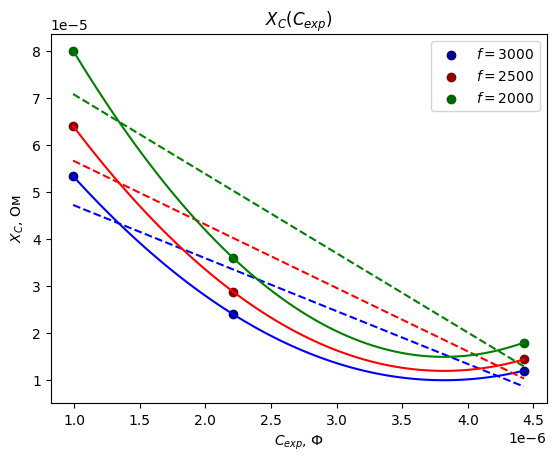
\includegraphics[scale=0.8]{media/graph14a}
		\end{center}
		\caption{Графік залежності імпедансу $X_C$ від ємності $C$}
		\label{Picture_2}
	\end{figure}\newpage
   
\begin{figure}[h!]
		\begin{center}
			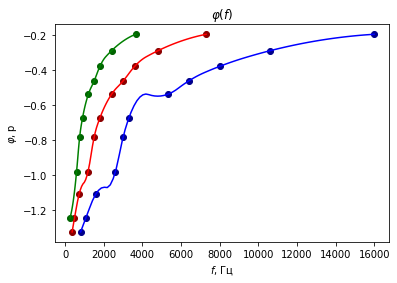
\includegraphics[scale=0.8]{media/graph15a}
		\end{center}
		\caption{Графік залежності зсуву фаз від частоти}
		\label{Picture_е}
	\end{figure}
	
\begin{table}[htp]
    \begin{flushright}
		\caption{Залежності зсуву фаз від частот в усіх даних }
	\end{flushright}
\centering
\begin{tabular}{|c|c|c|c|c|c|c|}
\hline
   & $X_C$, Ом& $f$, Гц & $C$, Ф& $R$, Ом& $\tan\varphi$ & $\varphi$, р\\ \hline
0  & 200   & 800   & 1   & 50  & -4.0          & -1.33     \\ \hline
1  & 150   & 1060  & 1   & 50  & -3.0          & -1.25     \\ \hline
2  & 100   & 1600  & 1   & 50  & -2.0          & -1.11     \\ \hline
3  & 75    & 2600  & 1   & 50  & -1.5          & -0.98     \\ \hline
4  & 50    & 3000  & 1   & 50  & -1.0          & -0.79     \\ \hline
5  & 40    & 3300  & 1   & 50  & -0.8          & -0.67     \\ \hline
6  & 30    & 5300  & 1   & 50  & -0.6          & -0.54     \\ \hline
7  & 25    & 6400  & 1   & 50  & -0.5          & -0.46     \\ \hline
8  & 20    & 8000  & 1   & 50  & -0.4          & -0.38     \\ \hline
9  & 15    & 10600 & 1   & 50  & -0.3          & -0.29     \\ \hline
10 & 10    & 16000 & 1   & 50  & -0.2          & -0.2      \\ \hline
\end{tabular}
\end{table}
\begin{table}[htp]
\centering
\begin{tabular}{|c|c|c|c|c|c|c|}
\hline
   & $X_C$, Ом& $f$, Гц & $C$, Ф& $R$, Ом& $\tan\varphi$ & $\varphi$, р\\ \hline
0  & 200   & 360  & 1   & 50  & -4.0          & -1.33     \\ \hline
1  & 150   & 480  & 1   & 50  & -3.0          & -1.25     \\ \hline
2  & 100   & 730  & 1   & 50  & -2.0          & -1.11     \\ \hline
3  & 75    & 1180 & 1   & 50  & -1.5          & -0.98     \\ \hline
4  & 50    & 1500 & 1   & 50  & -1.0          & -0.79     \\ \hline
5  & 40    & 1800 & 1   & 50  & -0.8          & -0.67     \\ \hline
6  & 30    & 2400 & 1   & 50  & -0.6          & -0.54     \\ \hline
7  & 25    & 3000 & 1   & 50  & -0.5          & -0.46     \\ \hline
8  & 20    & 3600 & 1   & 50  & -0.4          & -0.38     \\ \hline
9  & 15    & 4800 & 1   & 50  & -0.3          & -0.29     \\ \hline
10 & 10    & 7300 & 1   & 50  & -0.2          & -0.2      \\ \hline
\end{tabular}
\end{table}
\begin{table}[htp]
\centering
\begin{tabular}{|c|c|c|c|c|c|c|}
\hline
   & $X_C$, Ом& $f$, Гц & $C$, Ф& $R$, Ом& $\tan\varphi$ & $\varphi$, р\\ \hline
0  & 200   & 180   & 1   & 50  & -4.0          & -1.33     \\ \hline
1  & 150   & 240   & 1   & 50  & -3.0          & -1.25     \\ \hline
2  & 100   & 365   & 1   & 50  & -2.0          & -1.11     \\ \hline
3  & 75    & 590   & 1   & 50  & -1.5          & -0.98     \\ \hline
4  & 50    & 750   & 1   & 50  & -1.0          & -0.79     \\ \hline
5  & 40    & 900   & 1   & 50  & -0.8          & -0.67     \\ \hline
6  & 30    & 1200  & 1   & 50  & -0.6          & -0.54     \\ \hline
7  & 25    & 1500  & 1   & 50  & -0.5          & -0.46     \\ \hline
8  & 20    & 1800  & 1   & 50  & -0.4          & -0.38     \\ \hline
9  & 15    & 2400  & 1   & 50  & -0.3          & -0.29     \\ \hline
10 & 10    & 3650  & 1   & 50  & -0.2          & -0.2      \\ \hline
\end{tabular}
\end{table}\newpage
\subsection*{Висновок 1}
За результатами обробки дослідних даних отримано залеженість імпедансу від частоти, імпедансу від ємності, зсуву фаз від частоти та обраховано апроксимовану ємність:
\begin{itemize}
		\item $C_{\textrm{апр}}=0.993\cdot10^{-6}$
		\item $C_{\textrm{апр}}=2.214\cdot10^{-6}$
		\item $C_{\textrm{апр}}=4.428\cdot10^{-6}$
	\end{itemize}
Що майже відповідає номіналу. Таке незначне відхилення $(\langle\varepsilon_C\rangle=0.65\%)$, можливо, зумовлено різними наближеннями числа $\pi$ або неточністю вимірювань.\newpage
\subsection*{Частина 2} 
\begin{figure}[h!]
		\begin{center}
			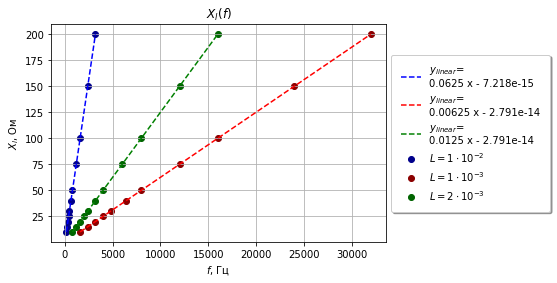
\includegraphics[scale=0.8]{media/graph16}
		\end{center}
		\caption{Графік залежності опору від частоти}
		\label{Picture_1}
	\end{figure}
	За допомогою формули (3) розрахуємо $L$ апроксимоване:
	\begin{equation}
		L_{\textrm{апр}}=\dfrac{k}{2\pi}
	\end{equation}
	де $b$ взято з формули апроксимації $y=k+{b}{x}$.
	\begin{itemize}
		\item $L_{\textrm{апр}}=\dfrac{0.0625}{2\pi}=9.947\cdot10^{-3}$
		\item $L_{\textrm{апр}}=\dfrac{0.00625}{2\pi}=0.994\cdot10^{-3}$
		\item $L_{\textrm{апр}}=\dfrac{0.0125}{2\pi}=1.989\cdot10^{-3}$
	\end{itemize}
	Також обрахуємо імпеданс за формулою (4).
	\begin{equation}
		X_L=\dfrac{f}{k}
	\end{equation}
\begin{table}[htp]
	\begin{flushright}
		\caption{Значення експериментальної індуктивності конденсатора та обчислення похибок}
	\end{flushright}
\begin{tabular}{|c|c|c|c|c|c|c|c|c|}
\hline
  & $k$     & $L_{\textrm{теор}}$, Гн & $L_{\textrm{апр}}$, Гн & $\Delta_L$, Гн     & $\varepsilon_L$ & $X_{L_1}$, Ом & $X_{L_2}$, Ом & $X_{L_3}$, Ом \\ \hline
0 & 0.0625  & $10\cdot10^{-3}$        & $9.947\cdot10^{-3}$    & $5.2\cdot10^{-5}$  & 0.5\%           & 187.5         & 156.25        & 125.0         \\ \hline
1 & 0.00625 & $1\cdot10^{-3}$         & $0.994\cdot10^{-3}$    & $5.2\cdot10^{-6}$  & 0.5\%           & 18.75         & 15.625        & 12.5          \\ \hline
2 & 0.0125  & $2\cdot10^{-3}$         & $1.989\cdot10^{-3}$    & $1.05\cdot10^{-6}$ & 0.5\%           & 37.5          & 31.25         & 25.0          \\ \hline
\end{tabular}
\end{table}
    
    \begin{figure}[h!]
		\begin{center}
			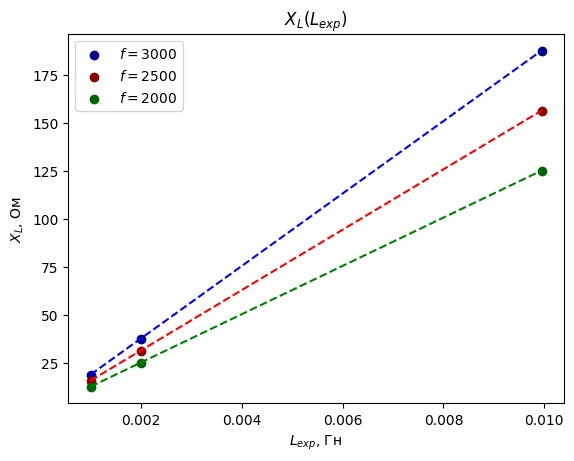
\includegraphics[scale=0.8]{media/graph17}
		\end{center}
		\caption{Графік залежності імпедансу $X_L$ від індуктивності $L$}
		\label{Picture_2}
	\end{figure}\newpage
   
\begin{figure}[h!]
		\begin{center}
			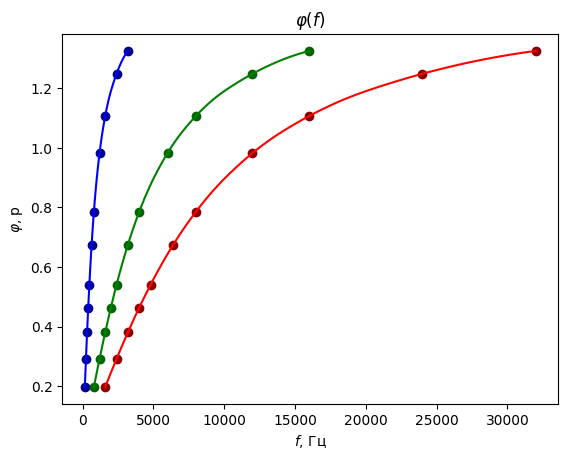
\includegraphics[scale=0.8]{media/graph18}
		\end{center}
		\caption{Графік залежності зсуву фаз від частоти}
		\label{Picture_е}
	\end{figure}
	
\begin{table}[htp]
\begin{flushright}
		\caption{Залежності зсуву фаз від частот в усіх даних }
	\end{flushright}
\centering

\begin{tabular}{|c|c|c|c|c|c|c|}
\hline
   & $X_L$, Ом & $f$, Гц & $L$, Гн & $R$, Ом & $\tan\varphi$ & $\varphi$, р \\ \hline
0  & 10        & 160     & 1       & 50      & 0.2           & 0.2          \\ \hline
1  & 15        & 240     & 1       & 50      & 0.3           & 0.29         \\ \hline
2  & 20        & 320     & 1       & 50      & 0.4           & 0.38         \\ \hline
3  & 25        & 400     & 1       & 50      & 0.5           & 0.46         \\ \hline
4  & 30        & 480     & 1       & 50      & 0.6           & 0.54         \\ \hline
5  & 40        & 640     & 1       & 50      & 0.8           & 0.67         \\ \hline
6  & 50        & 800     & 1       & 50      & 1.0           & 0.79         \\ \hline
7  & 75        & 1200    & 1       & 50      & 1.5           & 0.98         \\ \hline
8  & 100       & 1600    & 1       & 50      & 2.0           & 1.11         \\ \hline
9  & 150       & 2400    & 1       & 50      & 3.0           & 1.25         \\ \hline
10 & 200       & 3200    & 1       & 50      & 4.0           & 1.33         \\ \hline
\end{tabular}
\end{table}  
\begin{table}[htp]
\centering
\begin{tabular}{|c|c|c|c|c|c|c|}
\hline
   & $X_L$, Ом & $f$, Гц & $L$, Гн & $R$, Ом & $\tan\varphi$ & $\varphi$, р \\ \hline
0  & 10        & 1600    & 1       & 50      & 0.2           & 0.2          \\ \hline
1  & 15        & 2400    & 1       & 50      & 0.3           & 0.29         \\ \hline
2  & 20        & 3200    & 1       & 50      & 0.4           & 0.38         \\ \hline
3  & 25        & 4000    & 1       & 50      & 0.5           & 0.46         \\ \hline
4  & 30        & 4800    & 1       & 50      & 0.6           & 0.54         \\ \hline
5  & 40        & 6400    & 1       & 50      & 0.8           & 0.67         \\ \hline
6  & 50        & 8000    & 1       & 50      & 1.0           & 0.79         \\ \hline
7  & 75        & 12000   & 1       & 50      & 1.5           & 0.98         \\ \hline
8  & 100       & 16000   & 1       & 50      & 2.0           & 1.11         \\ \hline
9  & 150       & 24000   & 1       & 50      & 3.0           & 1.25         \\ \hline
10 & 200       & 32000   & 1       & 50      & 4.0           & 1.33         \\ \hline
\end{tabular}
\end{table}
\begin{table}[htp]
\centering
\begin{tabular}{|c|c|c|c|c|c|c|}
\hline
   & $X_L$, Ом & $f$, Гц & $L$, Гн & $R$, Ом & $\tan\varphi$ & $\varphi$, р \\ \hline
0  & 10        & 800     & 1       & 50      & 0.2           & 0.2          \\ \hline
1  & 15        & 1200    & 1       & 50      & 0.3           & 0.29         \\ \hline
2  & 20        & 1600    & 1       & 50      & 0.4           & 0.38         \\ \hline
3  & 25        & 2000    & 1       & 50      & 0.5           & 0.46         \\ \hline
4  & 30        & 2400    & 1       & 50      & 0.6           & 0.54         \\ \hline
5  & 40        & 3200    & 1       & 50      & 0.8           & 0.67         \\ \hline
6  & 50        & 4000    & 1       & 50      & 1.0           & 0.79         \\ \hline
7  & 75        & 6000    & 1       & 50      & 1.5           & 0.98         \\ \hline
8  & 100       & 8000    & 1       & 50      & 2.0           & 1.11         \\ \hline
9  & 150       & 12000   & 1       & 50      & 3.0           & 1.25         \\ \hline
10 & 200       & 16000   & 1       & 50      & 4.0           & 1.33         \\ \hline
\end{tabular}
\end{table}
\newpage
\subsection*{Висновок 2}
За результатами обробки дослідних даних отримано залеженість імпедансу від частоти, імпедансу від індуктивності, зсуву фаз від частоти та обраховано апроксимовану індуктивність:
\begin{itemize}
		\item $L_{\textrm{апр}}=9.947\cdot10^{-3}$
		\item $L_{\textrm{апр}}=0.994\cdot10^{-3}$
		\item $L_{\textrm{апр}}=1.989\cdot10^{-3}$
	\end{itemize}
Що майже відповідає номіналу. Таке незначне відхилення $(\langle\varepsilon_L\rangle=0.5\%)$, можливо, зумовлено різними наближеннями числа $\pi$ або неточністю вимірювань.\newpage
    
    
    
    
    
    
    
    
    
    
    
    
    
    
    
    
    
    
    
    
    
    
    
    
    
    
    
    
    
    
    
\end{justify}


\end{document}